\documentclass[11pt,a4paper]{article}
\usepackage{fontspec}\setmainfont{Noto Serif CJK SC}\setsansfont{Noto Sans CJK SC}\setmonofont{DejaVu Sans Mono}
\XeTeXlinebreaklocale "zh"\XeTeXlinebreakskip=0pt plus 1pt
\usepackage[margin=22mm]{geometry}\usepackage{amsmath,amssymb,booktabs,graphicx,hyperref,fancyhdr}
\hypersetup{pdftitle={LTN周期接触oracle三档物质空间对照},pdfauthor={diffuse-mixing research},colorlinks=true,urlcolor=blue}
\setlength{\parindent}{0pt}\setlength{\parskip}{6pt}\setlength{\headheight}{16pt}
\pagestyle{fancy}\fancyhf{}\fancyhead[L]{\small diffuse-mixing / LTN}\fancyhead[R]{\small 2026-11-04}\fancyfoot[C]{\thepage}
\begin{document}
\begin{center}{\LARGE\bfseries LTN扩散与掺混}\par\vspace{3mm}{\Large 周期接触oracle三档物质空间对照}\par\vspace{3mm}2026年11月4日（Asia/Shanghai）\end{center}
\section*{1. 本轮结论与固定问题}
\textbf{N16/32/64同一普通点FV静止周期接触的空间对照通过。Stage 3仍未完整通过，fluid ORC关闭，κ未计算。}

本轮严格执行上一轮唯一登记项：同一单位周期方形、等半两相$\rho_L=1,\rho_R=4$、原二进制$D=0.02$、$T=1/20$、$K=16$不变。只补N16/N64两张静态点图与两条实际/完整独立路径，N32全部保存状态只加载、不重算。静态$L$无中点冻结时间误差，不制造4/8/16时间阶，不继续N128或角度/模型扫描。

\textbf{两个时刻、两相邻档的原生/共同浓度与原生/共同H误差改善均超过预定正项指标。} 三项新增软件检查、主计算和完整独立审计首次通过。旧493项检查未重跑，累计记录496项，不冒称恢复旧v0.8.0/246。

\subsection*{真实物质状态与独立实现}
\[
m_i=\int_{K_i}\rho\,dV,\qquad
\bar c_i=\frac1{m_i}\int_{K_i}\rho c\,dV,\qquad m_i=\frac{\rho_i}{N^2}.
\]
原连续初场按每档有限单元积分新推导，不插值旧平均或从轨迹点值重采样。两个新系数图全部先封存，再加载质量、c0、参考或旧状态。构图仅收点、ID、给定oracle点密度、D及周期边界；不收真实物质面、参考或F/C。
\[
g_{ij}=\frac{|f_{ij}|}{\ell_i/(\rho_iD)+\ell_j/(\rho_jD)},\quad
g_L=D,\quad g_R=4D,\quad g_{LR}=\frac85D.
\]
上式仅在封存后逐面核对。原点Voronoi、普通阻力、稀疏指数/统一化、时序及H实现全部字节不改；没有裁剪、删除正面、归一化或阈值调整。

各档复用原128模态90位连续系数，Decimal100/120评价真实均值，独立mpmath80/100核验。初态直接积分原公式，两个正时刻分别核算尾项，保留所有初态/序列化桥。独立Cartesian控制保留全部离散模态与原始负零特征值；两新网格各17端点用独立Padé指数核对。

\subsection*{同一N16物质区域上的公平观测}
\[
(Pc)_I=\frac{\sum_{i\subset I}m_i c_i}{m_I^{(16)}},\qquad
\sigma_{0,16}=0.1961821193294627,\qquad H=1-\frac{\mathrm{Var}_m(c)}{\mathrm{Var}_m(c_0)}.
\]
容量逐块核对，不修补质量或均值。跨网格误差比较固定上述区域与分母，原生误差另列自身分母；各自H分别与各自参考比较，避免混淆不同观测。所有容量因子、初态及参考聚合桥保留。
\newpage
\section*{2. 三档结果与固定正项比较}
\begin{center}\small\begin{tabular}{rrrrr}\toprule
N & $t$ & 原生误差/自身$\sigma_0$ & 共同误差/N16$\sigma_0$ & 共同H误差\\\midrule
16 & 0.025 & 0.001295163 & 0.001295163 & 0.0007136686 \\
16 & 0.05 & 0.001763062 & 0.001763062 & 0.001326202 \\
32 & 0.025 & 0.0003291369 & 0.0003253732 & 0.0001809686 \\
32 & 0.05 & 0.0004341108 & 0.0004177902 & 0.0003366225 \\
64 & 0.025 & 8.135736e-05 & 7.741353e-05 & 4.603247e-05 \\
64 & 0.05 & 0.0001088427 & 0.0001024957 & 8.458189e-05 \\
\bottomrule\end{tabular}\end{center}
终时共同误差：$1.76306246\times10^{-3}$、$4.17790234\times10^{-4}$、$1.02495677\times10^{-4}$。相邻误差比约4.220和4.076，仅是本例观察，不拟合或认证一般收敛阶，不外推浓度。
\begin{center}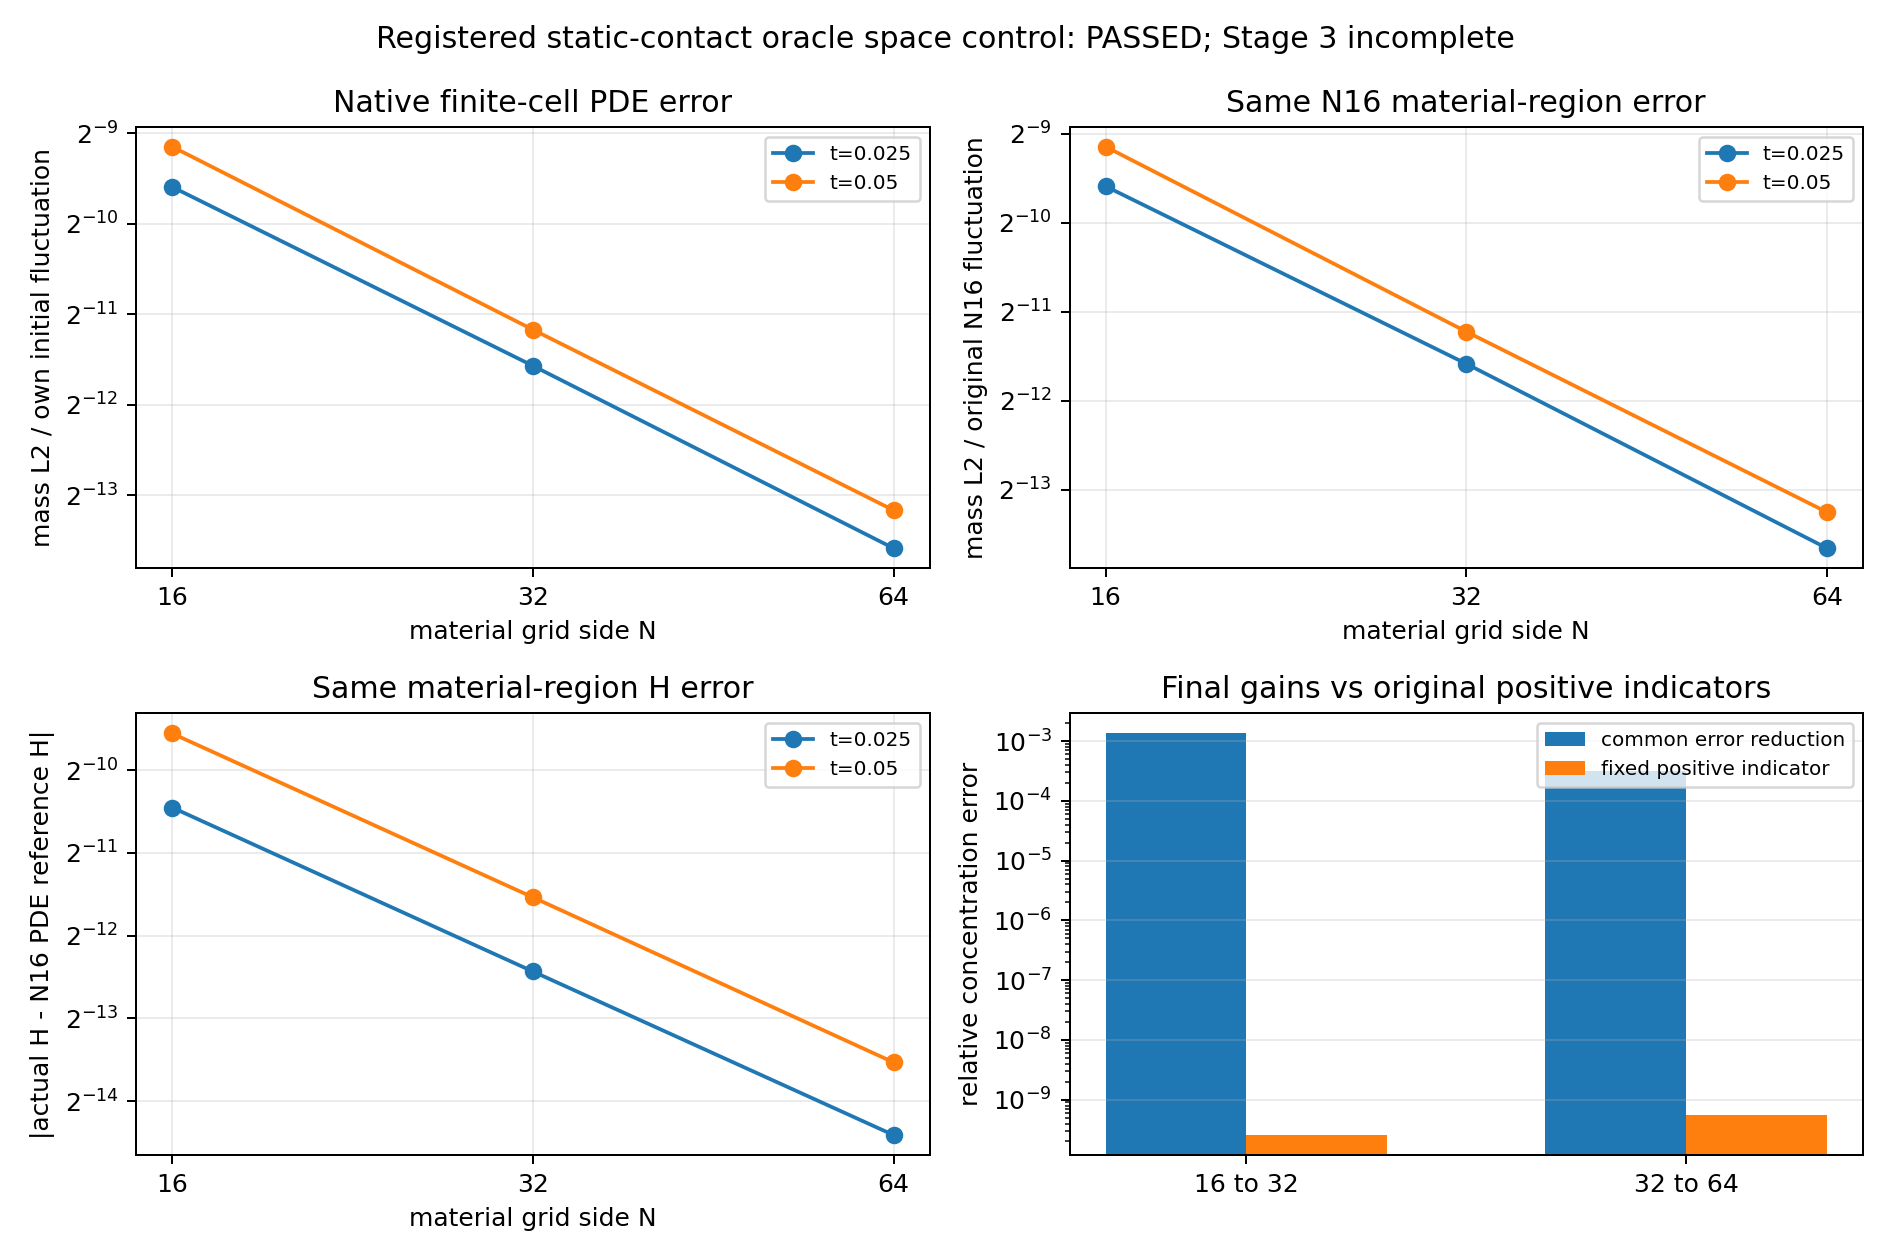
\includegraphics[width=.98\textwidth]{contact-spatial.png}\end{center}
\begin{center}\small\begin{tabular}{rrrr}\toprule
相邻档 & $t$ & 共同误差改善 & 固定正项指标\\\midrule
16→32 & 0.025 & 0.000969789 & 1.30108e-10 \\
16→32 & 0.05 & 0.00134527 & 2.56632e-10 \\
32→64 & 0.025 & 0.00024796 & 2.8347e-10 \\
32→64 & 0.05 & 0.000315295 & 5.60502e-10 \\
\bottomrule\end{tabular}\end{center}
所有原生/共同浓度及原生/共同H四量均要求改善超过各自指标，不能只挑上表中共同误差放行。预算保留双方原机器/尾项、完整序列差、Cartesian谱/变换/舍入、评价、参考截断与序列化及初态桥；共同观测乘容量因子并加所有投影桥。H对数值项用原二次h\_indicator并加直接绝对H桥，无有符号抵消。
\newpage
\section*{3. 验证、保全与下一步}
三项必要软件检查首次通过：多N精确界面g及独立Gauss有限均值；不等子质量直接积分与非零桥保留；正项分类、完整序列损坏及细格高频误差被共同聚合掩盖时的原生控制拒绝。\textbf{原生可分辨变差即拒绝，即使共同观测改善。}

主计算首次11.662秒／89.62 MiB，满足900秒／1024 MiB封顶。完整独立审计首次31.944秒／83.16 MiB通过。两新图均独立重建双中垂线/互反面/半阻力/面积/固定全点探针；精确率、最小$10^{-16}$ Poisson尾项、原权重与全部独立序列逐位核对，原始库存/极值/方差/耗散按原尺度核验。

共同物质审计不调用生产聚合函数：独立分ID并直接核验165份快照和825个Fraction母单元积分探针，最大fsum与保存均值差$2.22\times10^{-16}$。N32原判别及其首次失败/类型恢复记录保持，不覆盖旧结果。

782原文件、15附件、100份先前正式科学清单保持；四份历史诊断既有差异保留。原README/METHOD/CODEX\_TASK/PHASE与旧代码/数据/报告不改，仅更新研究状态入口及备份交接文件。PDF/代码ZIP和GitHub备份延续用户已授权范围，不是环境或版本发布。

\subsection*{唯一下一项：移动Becker物理接口与单例}
静止周期接触三档oracle控制已完成，剩余T4缺口是最终同一后端的移动激波与三密度来源闭合。下一项先写两个具体接口契约，再执行一个原Becker oracle判别：
\begin{itemize}
\item 给定移动最外物质端点的x零通量边界，y单位周期；不把激波当固壁、不把x做周期，不能向点构造器提供真实内部物质面。
\item T显式的可选时序包装，共享原指数/统一化与H。现helper硬编码T=.05，不能直接用于T=.1；新包装须先在T=.05夹具逐位匹配旧路径。
\item 固定$\delta=.08,D=.02,T=.1$、原32物质列，横向复制8行；点沿固定质量标签中点轨迹，不强迫成真实单元几何中心。复用原质量/c0与已保存8192空间/时间参考，不新解PDE。
\end{itemize}
本轮仅绑定来源SHA，未生成新Becker点、图、状态或参考评价。接口/算例失败或未分辨则保留停止，不调代表位置、网格或阈值制造通过。oracle单例不代表kernel/ledger密度已验收，fluid ORC继续关闭。

\subsection*{恢复与重放}
ZIP含研究代码/文档、782原始文件、本轮三档状态/系数/参考/审计，以及下一步Becker精选已存来源；不含完整约39GB工作区或15附件。完整历史保全审计仍需原工作区。新解压目录可重放两条新路径，N32只加载：
\begin{quote}\small\begin{verbatim}
OPENBLAS_NUM_THREADS=4 OMP_NUM_THREADS=4 \
PYTHONDONTWRITEBYTECODE=1 python \
research/reconnect/contact_spatial_study.py \
--replay runs/reconnect-contact-spatial
\end{verbatim}\end{quote}
逐位重放与平台/数值库构建有关；不一致时保留差异，不放宽物理阈值。文件CRC/SHA、新解压和GitHub克隆核验以交付收据为准。Stage3 incomplete，κ未算。
\end{document}
